\documentclass[a4paper,10pt]{article}
\usepackage{amsmath}
\usepackage{amssymb}
\usepackage[polish]{babel}
\usepackage{polski}
\usepackage[utf8]{inputenc}
\usepackage{indentfirst}
\usepackage{geometry}
\usepackage{array}
\usepackage[pdftex]{color,graphicx}
\usepackage{subfigure}
\usepackage{afterpage}
\usepackage{setspace}
\usepackage{color}
\usepackage{wrapfig}
\usepackage{listings}
\usepackage{datetime}

\renewcommand{\onehalfspacing}{\setstretch{1.6}}

\geometry{tmargin=2.5cm,bmargin=2.5cm,lmargin=2.5cm,rmargin=2.5cm}
\setlength{\parindent}{1cm}
\setlength{\parskip}{0mm}

\newenvironment{lista}{
\begin{itemize}
  \setlength{\itemsep}{1pt}
  \setlength{\parskip}{0pt}
  \setlength{\parsep}{0pt}
}{\end{itemize}}

\newcommand{\linia}{\rule{\linewidth}{0.4mm}}

\definecolor{lbcolor}{rgb}{0.95,0.95,0.95}
\lstset{
    backgroundcolor=\color{lbcolor},
    tabsize=4,
  language=C++,
  captionpos=b,
  tabsize=3,
  frame=lines,
  numbers=left,
  numberstyle=\tiny,
  numbersep=5pt,
  breaklines=true,
  showstringspaces=false,
  basicstyle=\footnotesize,
  identifierstyle=\color{magenta},
  keywordstyle=\color[rgb]{0,0,1},
  commentstyle=\color{Darkgreen},
  stringstyle=\color{red}
  }

\begin{document}

\noindent
\begin{tabular}{|c|p{11cm}|c|} \hline 
L2 & Przemysław Kleszcz, Krzysztof Tatar & \ddmmyyyydate\today \tabularnewline
\hline 
\end{tabular}


\section*{Zadanie 3 - Rozmycie Gaussa w CUDA}

Celem zadania było napisanie programu, który rozmywa zadane zdjęcie za pomocą algorytmu Gaussa z maską o wymiarach 5x5. Do poprawnego działania programu należy podać dwa argumenty wejściowe. Są to \emph{input\_image - ścieżka do pliku obrazu w formacie JPEG} i \emph{output\_image - ścieżka do pliku wyjściowego obrazu w formacie JPEG
}.Poniżej przedstawiony jest rysunek zastosowanej filtracja na podstawie filtra o masce 5 x 5 wraz z wagami, które są wykorzystywane podczas przeprowadzania obliczeń.

\begin{figure}[!ht]
	\centering
 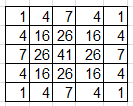
\includegraphics[width=0.2\textwidth]{3.png}
  \caption{Wykorzystana maska Gaussowska}
\end{figure}

Poniżej zaprezentowano główną funkcję programu odpowiedzialną za zrównoleglanie obliczeń.

\begin{lstlisting}
__global__
void gaussian(uchar * picture, uchar * pictureNew, long sizeX, long sizeY)
{
	int mask[5][5] = 
	{
		{ 1,4 ,7 ,4 ,1 },
		{ 4,16,26,16,4 },
		{ 7,26,41,26,7 },
		{ 4,16,26,16,4 },
		{ 1,4 ,7 ,4 ,1 }
	};
	int weight = 273;
	long x = blockIdx.x * blockDim.x + threadIdx.x;
	long y = blockIdx.y * blockDim.y + threadIdx.y;

	if (x < sizeX - 2 && y < sizeY - 2 && x>1 && y>1)
	{
		long r = 0, g = 0, b = 0;
		long wInput, wOutput;

		for (int i_y = 0; i_y < 5; i_y++) 
		{
			for (int i_x = 0; i_x < 5; i_x++) 
			{
				wInput = sizeX * (y + i_y - 2) * 3 + (x + i_x - 2) * 3;
				r += picture[wInput + 2] * mask[i_x][i_y];
				g += picture[wInput + 1] * mask[i_x][i_y];
				b += picture[wInput] * mask[i_x][i_y];
			}
		}

		wOutput = (sizeX - 4)*(y - 2) * 3 + (x - 2) * 3;
		pictureNew[wOutput + 2] = r / weight;
		pictureNew[wOutput + 1] = g / weight;
		pictureNew[wOutput] = b / weight;
	}
}
\end{lstlisting}

W powyższym programie został zastosowany algorytm filtrowania za pomocą którego posiadamy możliwość rozmycia podanego obrazka. 
Do zrównoleglenia rozwiązania w kernelu zostało użyta strategia podziału na bloki oraz wątki. Do kernelu zostały przekazywane podział boków od 1 do 30 przy czym rozmiar bloków był 16.
\newline
Główne funcje CUDA
\begin{lstlisting}
 __global__
\end{lstlisting}
Kwalifikator \_\_global\_\_to dodatek pochodzący z języka CUDA C. Informuje on kompilator
o tym, że dana funkcja powinna zostać skompilowana dla urządzenia, a nie dla hosta. 
\newline
\begin{lstlisting}
	long x = blockIdx.x * blockDim.x + threadIdx.x;
	long y = blockIdx.y * blockDim.y + threadIdx.y; 
\end{lstlisting}
Ponieważ każdy wątek powinien rozpoczynać działanie od innego indeksu, musimy indeksy wątków i bloków przerobić na indeksy liniowe. Każdy wątek zostanie uruchomiony na danych znajdujących się pod indeksem obliczonym za pomocą powyższej instrukcji.
\newline
\begin{lstlisting}
	cudaEvent_t timeStart, timeEnd;
	float time;
	cudaEventCreate(&timeStart);
	cudaEventCreate(&timeEnd);
	cudaEventRecord(timeStart, 0);
	gaussian<<<grids, blocks>>>(devPicture, devPictureNew, picture.cols, picture.rows);
	cudaDeviceSynchronize();
	cudaEventRecord(timeEnd, 0);
	cudaEventSynchronize(timeEnd);
	cudaEventElapsedTime(&time, timeStart, timeEnd);
\end{lstlisting}
Aby zmierzyć czas wykonywania bloku kodu, musimy utworzyć zdarzenie zarówno początku, jak
i końca. Najpierw nakażemy systemowi zarejestrować moment rozpoczęcia operacji, następnie damy
mu jakieś zadania do wykonania przez GPU, a na koniec zażądamy zakończenia rejestracji.
\begin{lstlisting}
cudaFree(devPicture);
cudaFree(devPictureNew);
\end{lstlisting}
Uwalnia przestrzeń pamięci wskazywaną przez wskaźnik.
\newline
\begin{lstlisting}
	cudaMalloc((void**)& devPicture, sizeIn);
	cudaMalloc((void**)& devPictureNew, sizeOut);
\end{lstlisting}
cudaMalloc alokuje pamięć na urzą­
dzeniu za pośrednictwem systemu wykonawczego CUDA.
\begin{lstlisting}
cudaMemcpy(pictureNew.data, devPictureNew, sizeOut, cudaMemcpyDeviceToHost)
\end{lstlisting}
Dodatkowo dostęp do pamięci urządzenia na hoście można uzyskać za pomocą funkcji
cudaMemcpy().
\begin{figure}[ht]
	\centering
  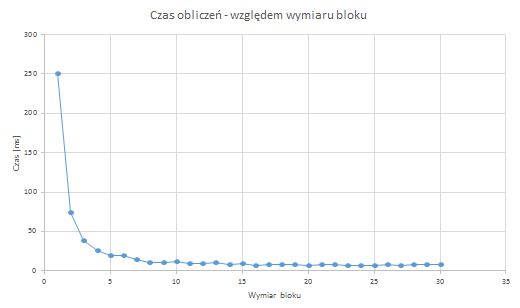
\includegraphics[width=0.7\textwidth]{2.png}
  \caption{Wykres przyspieszenia}
\end{figure}

Z powyższego rysunku można wywnioskować, że średni czas obliczeń dynamicznie malał dla pierwszych 5 bloków. Następnie dla podziału od 6 do 16 czas również delikatnie spada. Po następnym podziale od 17 do 30 już nie jest zauważalny spadek czasu obliczeń.

\end{document}
